\subsection{Configuration Export}

None of the \glspl{cpe} support exporting the configuration file on the standard \gls{http} Management Interface, even when signing in with the admin user. But a hidden interface is available in all devices and it allows the configuration file to be exported. To access this interface, you must navigate to \url{http://192.168.15.1/padrao} and log into the support user, using the admin’s password.

On \glspl{cpe} 2 to 7, you can navigate through the menu and export the configuration in the proper page with the support account. But \glspl{cpe} 0 and 1 don’t have the export page indexed in the menu, and you must access \url{http://192.168.15.1/saveconf.htm} manually, shown in Figure \ref{figure:cpe_saveconf}.

\begin{figure}[h]
    \centering
    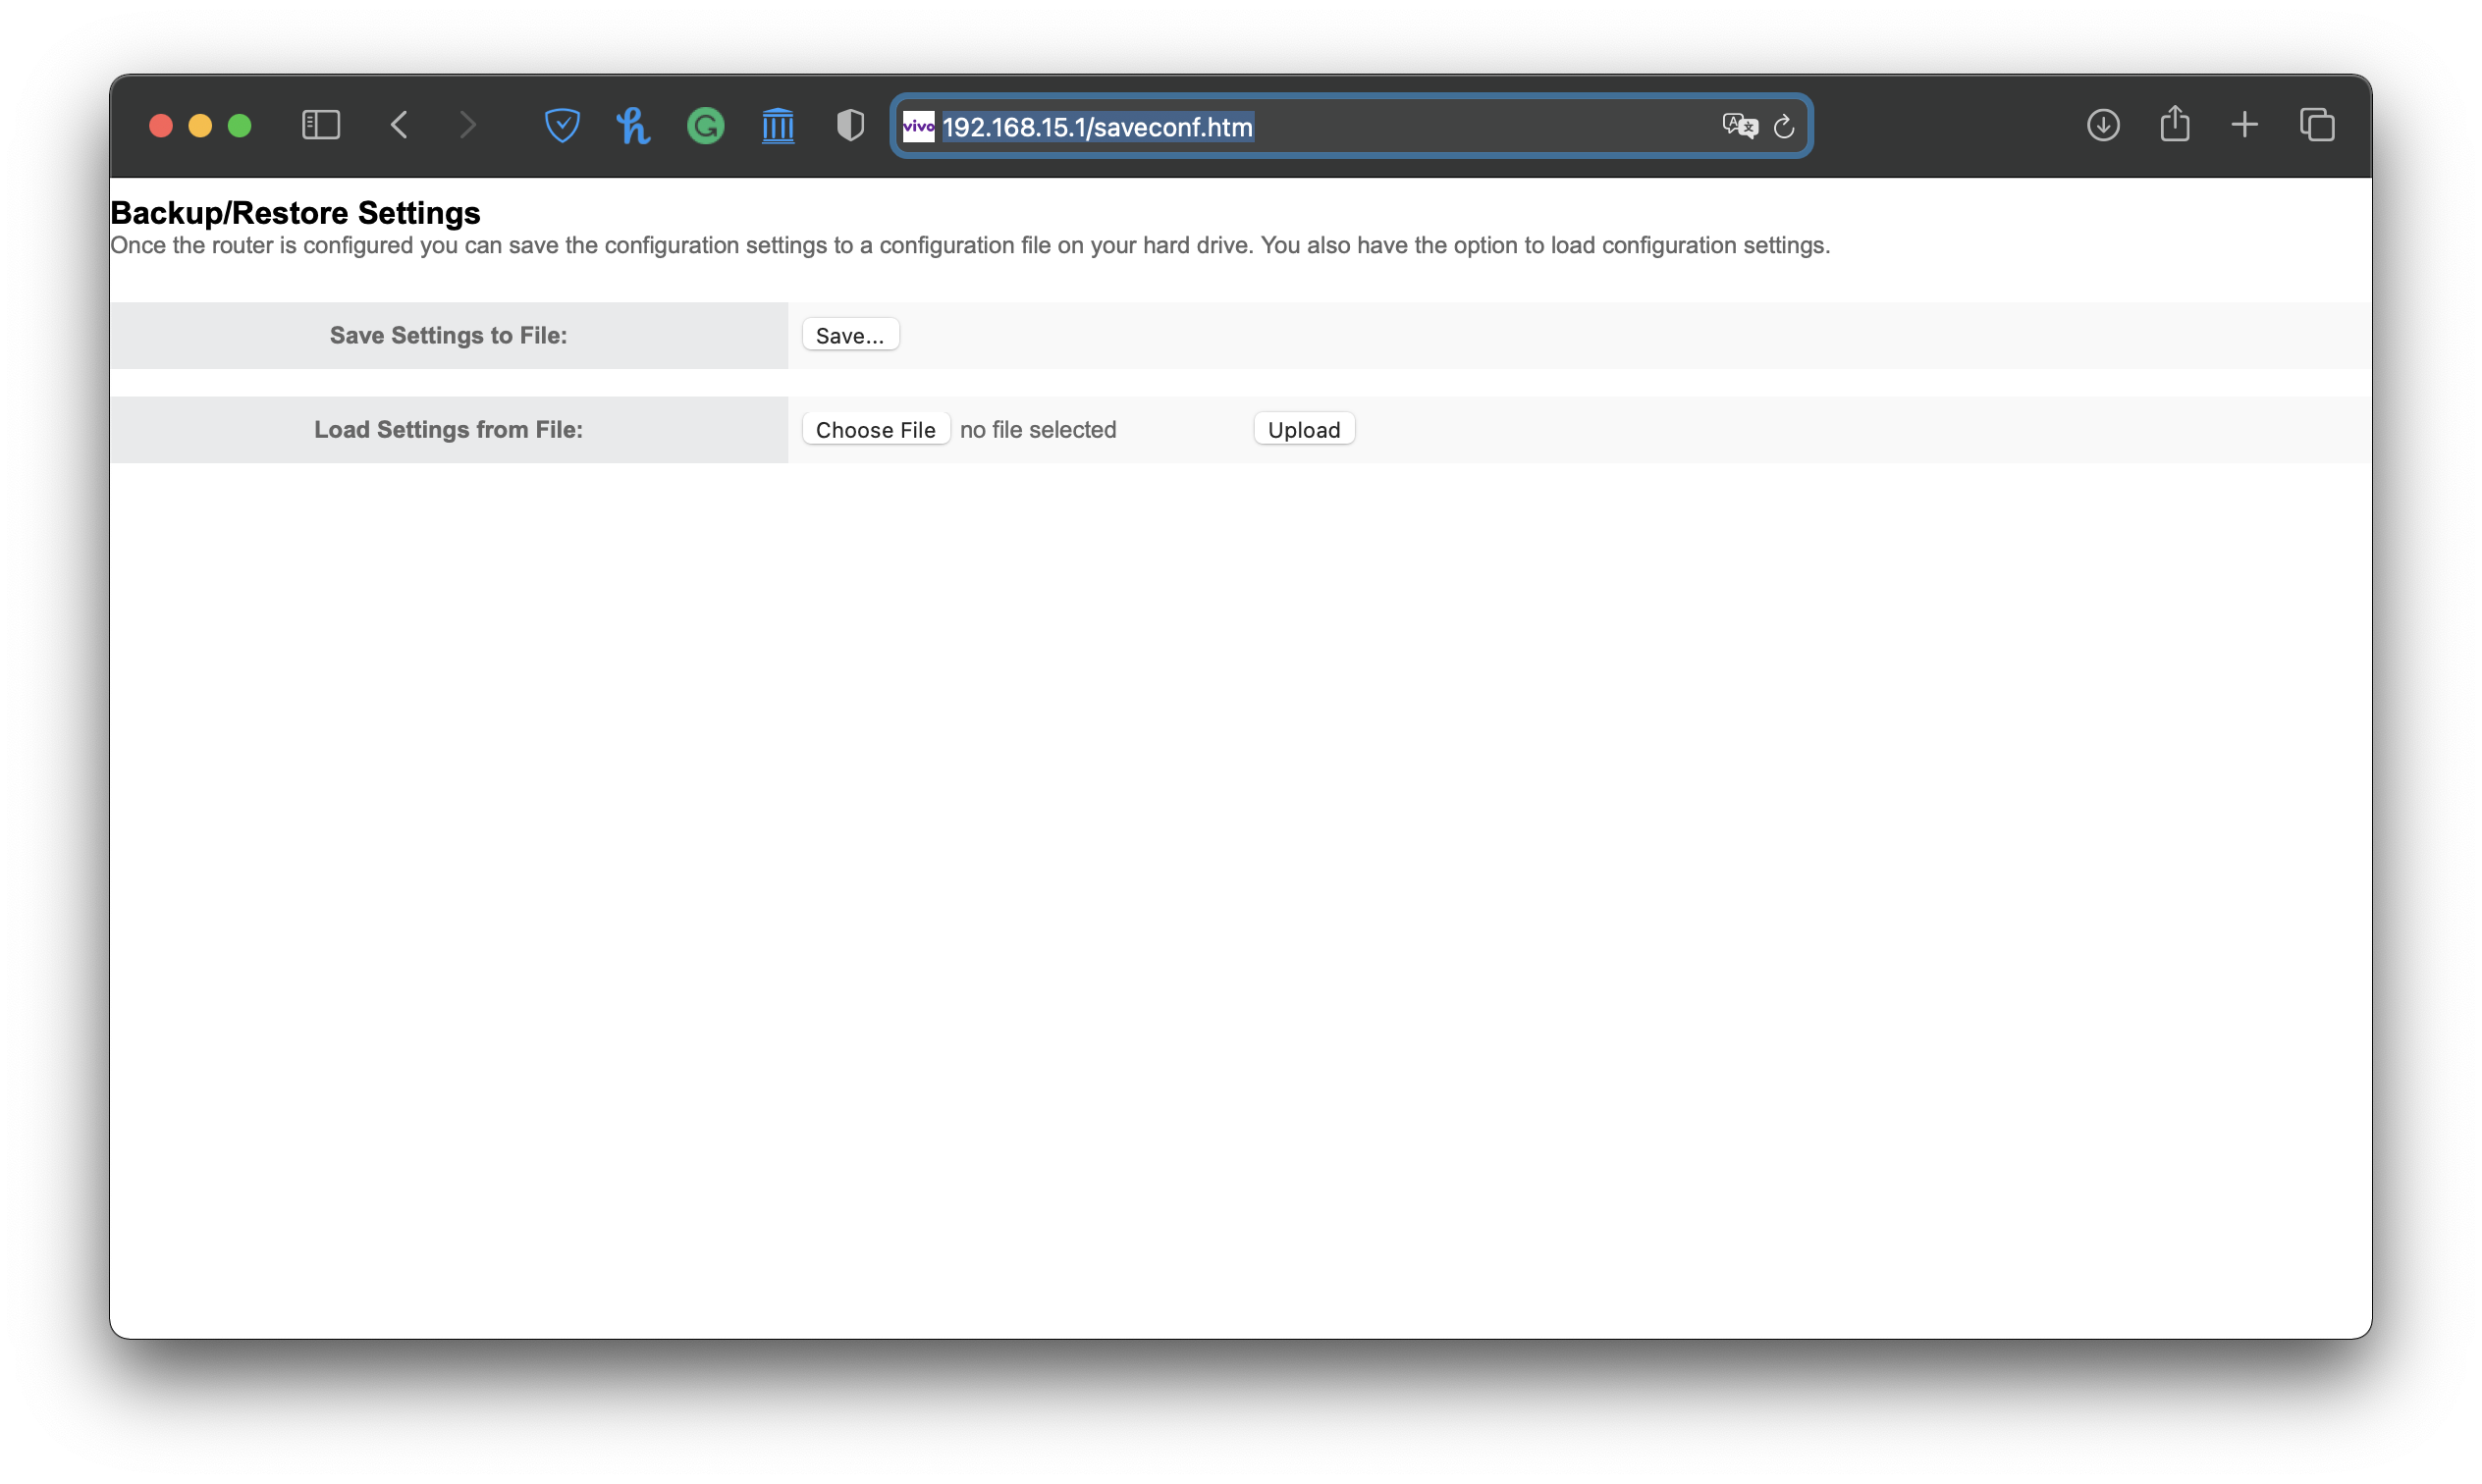
\includegraphics[width=\linewidth]{contents/cpes-and-research-data/configuration-export/cpe-saveconf.png}
    \caption{Unindexed \gls{cpe} Configuration Export Page}
    \label{figure:cpe_saveconf}
\end{figure}

\FloatBarrier
